\termin{10.06.2016}

\mdf{Definition}
Betrachtet man zwei stochastische Vorgänge mit Ergebnisräumen $\Omega _1$ und $\Omega _2$ kann man beide Vorgänge zu einem simultanen Vorgang zusammenführen. Dieser hat den Ergebnisraum
\begin{align*}
    \Omega = \Omega _1 \times \Omega _2 = \{(\omega _1, \omega _2) \,|\, \omega _1 \in \Omega _1, \omega _2 \in \Omega _2\}
\end{align*}
Sind $A_1 \subseteq \Omega _1, A_2 \subseteq \Omega _2$ Ereignisse, so bezeichnet das \begr{Produktereignis} $A = A_1 \times A_2$ das simultane Eintreten der beiden Einzelergebnisse $A_1$ und $A_2$. Die beiden stochastischen Vorgänge heißen \begr[Unabhängigkeit (Stochastik)]{unabhängig}, falls für alle $A_1 \subseteq \Omega _1, A_2 \subseteq \Omega _2$ gilt:
\begin{align*}
    P(A_1 \times A_2) = P(A_1) \cdot P(A_2)
\end{align*}
bzw. in Zufallsvariablen
\begin{align*}
    P\{X_1 \in A_1, X_2 \in A_2\} = P\{X_1 \in A_1\} \cdot P\{X_2 \in A_2\}
\end{align*}

\mdf{Beispiel}
Seien die beiden Zufallsvariablen $X_1$ = Augenzahl auf der oberen Seite eines Würfels und $X_2$ = gegenüberliegende Augenzahl. Es gilt $X_1 + X_2 = 7$, $X_1$ und $X_2$ sind nicht statistisch unabhängig.
\begin{align*}
    P\{X_1 = 1, X_2 = 6\} = \frac{1}{6} \neq P\{X_1 = 1\} \cdot P\{X_2 = 6\} = \frac{1}{6} \cdot \frac{1}{6} = \frac{1}{36}
\end{align*}
Hingegen sind $X_1$ = Augenzahl im 1. Wurf, $X_2$ = Augenzahl im 2. Wurf statistisch unabhängig.

\mdf{Satz}
Sind $X_1, X_2$ stochastisch unabhängig, so gilt $P\{X_2 \in A_2|X_1 \in A_1\} = P\{X_2 \in A_2\}$

\kapitel{Diskrete Zufallsvariablen}
Diskret bedeutet: $X$ nimmt nur isolierte Werte von Zahlen, den so genannten \begr{Träger} $T = \{x_1, x_2, \dots\}$, an. Elemente von $T$ heißen \begr{Realisierungen} von $X$ (oft $T \subseteq \mathbb{N}$). Ist $x \in T$, so heißt $P\{X = x\}$ \begr{Elementarwahrscheinlichkeit} für $x$.

\mdf{Satz}
$A = \{a_1, a_2, \dots\} \subseteq T$ sei ein Ereignis. Dann gilt
\begin{align*}
    P\{X \in A\} = \sum_{x \in A} P\{X = x\}
\end{align*}

\mdf{Definition}
Die Abbildung $\mathcal{P} \rightarrow [0, 1], A \mapsto P\{X \in A\}$ heißt \begr{Verteilung} von $X$. Bei diskreten Zufallsvariablen als Histogramm

\begin{center}
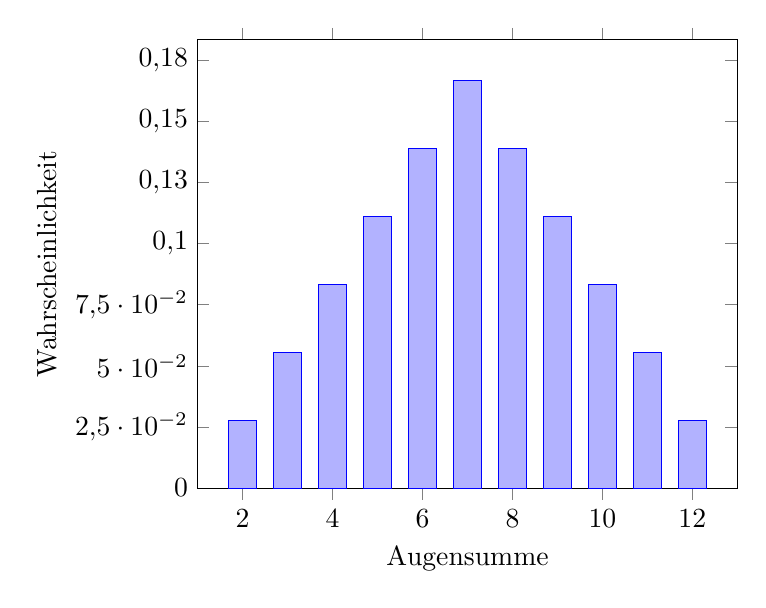
\begin{tikzpicture}
\begin{axis}[
    ybar,
    ymin=0,
    ytick={0,0.025,...,1},
    ylabel={Wahrscheinlichkeit},
    xlabel={Augensumme},
    /pgf/number format/.cd,
        use comma,
        1000 sep={}]
]
\addplot coordinates {(2,0.027777) (3,0.055556) (4,0.083333) (5,0.11111) (6,0.138888) (7,0.166667) (8,0.138888) (9,0.11111) (10,0.083333) (11,0.055556) (12,0.027777)};
\end{axis}
\end{tikzpicture}

Zweifacher Würfelwurf
\end{center}

\mdf{Definition}
Ist $T = \{x_1,\dots,x_n\}$ und sind die $n$ Realisierungen von $X$ alle gleich wahrscheinlich, so heißt $X$ diskret gleichverteil oder laplaceverteilt auf dem Träger $T$. Alle Elementarwahrscheinlichkeiten sind gleich. $P\{X = x_i\} = \frac{1}{n}$ für alle $i = 1,\dots,n$ und es gilt $P\{X \in A\} = \frac{|A|}{|T|} = \frac{|A|}{n}$, z.B. alle geraden Zahlen $= \frac{3}{6}$.

\bigskip
Betrachte stochastischen Vorgang und ein Ergebnis $A \subseteq \Omega$. Wir interessieren uns nun dafür, ob $A$ eintritt oder nicht. Wir reduzieren das Ergebnis unter Verwendung einer Indikatorenvariable $Y$.
\begin{align*}
    Y = \begin{cases}
        1 & \text{ falls $A$ eintritt (Treffer)} \\
        0 & \text{ falls $A$ nicht eintritt (Kein Treffer)/sonst}
    \end{cases}
\end{align*}
Wir bezeichnen die zugehörigen Wahrscheinlichkeiten mit
\begin{align*}
    p = P\{Y = 1\} = P(A) &\quad\text{ Trefferwahrscheinlichkeit} \\
    q = P\{Y = 0\} = 1 - P(A) = 1 - p &\quad\text{ nicht-Trefferwahrscheinlichkeit}
\end{align*}
Wir wiederholen den Vorgang statistisch unabhängig $n$-Mal. Dann ist die Anzahl $x$ der Treffer eine Zufallsvariable mit Träger $T = \{0,1,\dots,n\}$. Wie ist $x$ in Abhängigkeit von $n$, $p$ verteilt?

Sei $Y_i$ die Indikatorenvariable für einen Treffer im $i$-ten Vorgang. Dann ist $x = Y_1 + Y_2 + \dots + Y_n$ die Anzahl der Treffer.

\mdf{Satz}
Für die Elementarwahrscheinlichkeiten von $x$ gilt:
\begin{align*}
    P\{X = x\} = \begin{pmatrix}n\\x\end{pmatrix}p^xq^{n-x} = b(x|n,p)\text{ für }x\in T
\end{align*}

\mdf{Definition}
Die durch Satz 5 gegebene Verteilung von $a$ auf $\{0,1,\dots,n\}$ heißt \begr{Binomialverteilung} vom Umfang $n$ mit Trefferwahrscheinlichkeit $p$ und wird $B(n;p)$-Verteilung genannt.

\mdf{Korollar}
Die Anzahl der nicht-Treffer ist $B(n;q)$-verteilt.

\mdf{Lemma}
Für eine $B(n;p)$-verteilte Zufallsvariable $x$ gilt:
\begin{itemize}
    \item{$P\{X \leq x\} = P\{X = 0\} + P\{X = 1\} + \dots + P\{X = x\} = \sum_{k = 0}^x P\{X = k\}$}
    \item{$P\{X \geq x\} = \sum_{k = x}^{n} P\{X = k\}$}
    \item{$P\{x_1 \leq X \leq x_2\} = \sum_{k = x_1}^{x_2} P\{X = k\}$}
\end{itemize}

\mdf{Beispiel} (Wahlumfragen)

Anzahl $x$ der Befürworter der Partei ist $B(n;p) = B(100;0,08)$-verteilt. Wie hoch ist die Wahrscheinlichkeit, dass die Partei höchstens $5\%{}$ in der Umfrage erhält?

Berechne $P\{x \leq 5\} = P\{x = 0\} + P\{x = 1\} + \dots + P\{x = 5\} = 0,02\%{} + 0,21\%{} + 0,9\%{} + 2,54\%{} + 5,36\%{} + 8,96\%{} = 17,99\%{}$.
